This chapter covers the theory of the most widely used method for point prediction in the electricity forecasting literature. Besides discussing the theory underlying such models, this and the following chapter include also a couple of worked examples in order to get acquainted with the practical applications of these models.


% \section{Exponential smoothing}
% Exponential smoothing was developed by Brown \cite{brown1959statistical}, Holt \cite{holt1957forecasting}, Winters \cite{winters1960forecasting}.
% The idea is to forecast future values by taking a weighted average of past observations, where weights decay exponentially in time.
% \begin{equation}
%     \begin{aligned}
%         \hat{y}_{t+h|t}=& l_{t}+hb_{t}+s_{t+h-m(k+1)}
%         \\
%         l_t=&\alpha (y_t-s_{t-m})+(1-\alpha)(l_{t-1}+b_{t-1})
%         \\
%         b_t=& \beta(l_t-l_{t-1})+(1-\beta)b_{t-1}
%         \\
%         s_t=&\gamma(y_t-l_{t-1}-b_{t-1})+(1-\gamma)s_{t-m}
%     \end{aligned}
% \end{equation}
% where $0\leq \alpha \leq 1$ is the smoothing parameter and k is the integer part of $\frac{(h-1)}{m}$.%that is k encodes seasonalities
% Optimal parameters are obtained by minimising the sum of squared errors.


\section{Multiple linear regression}
Notwithstanding its simplicity, multiple linear regression models are still popular among the electricity point forecasting literature. Notice, they are not used per se but usually combined with other more advanced models.
\begin{equation}
    y_t=\beta X_t + \epsilon_t
\end{equation}

\section{Autoregressive models}
% explain their theory
% and how the procedure how they are used
% IMPORTANT: load series is not a stationary series so before applying AR we have to perform stationary tests or differencing steps
Autoregressive models are a standard approach for modelling time series data.
Before introducing the popular model in electricity point forecasting, it is important to remember that autoregressive models assume the time series to be stationary. On the other hand, load and price have been observed to be a non stationary time series. 
Basically, stationarity means that the distribution of any subsequence of random variables of the stochatic process is invariant to shifts along the time dimension.
Therefore, checking stationarity is a crucial step in applying this class of models. %(unit root tests)
Furthermore, should the time series be non stationary, we have to convert it to a stationary one by a combination of either differencing, detrending and/or log transforming it.
\subsection{Autoregressive integrated moving average}
ARIMA(p,d,q) models are of the form
\begin{equation}
    \hat{y}_n=\sum\limits_{i=1}^{p}\psi_i y_{n-i}^{(d)}+\sum\limits_{j=1}^{q}\theta_j \epsilon_{n-j}+\epsilon_n
\end{equation}
where the parameter p is the order of the autoregressive (AR) part, d is the degree of integrated differencing and q is the order of the moving average (MA) model. $\epsilon_{n-j}$ are the observed errors in the past while the differenced term $y_n^{(d)}$ is defined recursively as $y_n^{(d)}=y_n^{(d-1)}-y_{n-1}^{(d-1)}$.
\\
ARIMA model are compactly written as
\begin{equation}
    \psi(B)\nabla^d y_t=\theta(B)\epsilon_t
\end{equation}
where $B$ is the backward shift operator, $B^h y_t=y_{t-h}$ and $\psi(B)$ is shorthand for $\psi(B)=1-\psi_1B-\dots-\psi_p B^p$.
Similarly, $\theta(B)=1+\theta_1B+\dots+\theta_q B^q$ and $\nabla_h$ is the lag h differencing operator $\nabla_h y_t=(1-B^h)y_t=y_t-y_{t-h}$
\\
The most popular procedure for estimating this class of models is the Box-Jenkins method \cite{box2015time}.
The order p is identified by taking the lags at which the sample partial autocorrelation function (PACF) falls outside its 95\% confidence interval.
In the same way, the order q is estimated by considering the sample autocorrelation function of the observed time series. Finally, we compare ARIMA models with different p,d,q (in a neighbourhood of the identified orders) and choose the ones minimising either AIC or BIC criteria. 
% Notice, models are obtained through the maximum likelihood estimation framework.

\subsection{Autoregressive integrated moving average with exogenous variables}
ARIMAX model adds explanatory variables to our ARIMA, hence, we have
\begin{equation}
    \hat{y}_n=\sum\limits_{k=1}^{h} \mu_i X_{n-k}+\sum\limits_{i=1}^{p}\psi_i y_{n-i}^{(d)}+\sum\limits_{j=1}^{q}\theta_j \epsilon_{n-j}+ \epsilon_{n}
\end{equation}
\subsection{Seasonal autoregressive integrated moving average and Seasonal autoregressive integrated moving average with exogenous variables}
SARIMA and SARIMAX incorporate seasonalities into our time series models. The notation for these models is ARIMA$(p,d,q)(P,D,Q)_m$. The second term $(P,D,Q)_m$ represents the autoregressive structure of the seasonal patter, where $m$ indicates the number of seasonalities of our time series.
For instance, in modelling series of hourly data with daily periodicity, we would set m=24.
Writing SARIMA in compact notation we have
\\
\begin{equation}
    \psi(B)\Psi(B^s)\nabla^d\nabla_m^Dy_t=\theta(B)\Theta(B^s)\epsilon_t
\end{equation}
where $\Psi$ and $\Theta$ account for the $P$ and $Q$ of the seasonal patter $m$ respectively.
\section{Generalized additive model}
% in standard regression the predicted y are normal since error are normal. But if we want to model say a y bernoulli which is the rate of success we can link the domain of bernoulli to that of gaussian with a link function
Generalized additive models (GAMs) take the form
\begin{equation}
    g[\mathbb{E}(Y_i)]=\alpha+f_1(X_1)+\dots+f_p(X_p)
\end{equation}
$f_i$ are smooth functions which are fitted using cubic smoothing splines.
g is called link function and characterizes the specific GAM model \cite{hastie2017generalized}. Approximations for $f_i$ are obtained through an iterative procedure, the backfitting algorithm.

%prophet meta
Particularly successful in time series forecasting is the Prophet model \cite{taylor2018forecasting}, developed by Meta. This additive model is capable of handling non linear trends, holiday effects and yearly weekly and daily seasonality. Thus, the reason we choose it as a valid benchmark to compare against.
\section{K-nearest neighbours regression}
K-nearest neighbours regression forecasts by averaging the most similar k instances in the training set \cite{macqueen1967some}. K is the algorithm hyperparameter, it stands for the number of neighbours; a small k leads to overfitting while a big k leads to underfitting. 
Since it is a metric based algorithm, it is important to normalize data in order to give equal weights to features with different scales, see \ref{appendix:normalization}.
This algorithm is made up of two decisions: first, the choice of the metric and second, the method for combining targets.


\section{Support vector regression}
Developed at the AT\&T Bell Laboratories by Vapnik et al. \cite{cortes1995support} \cite{vapnik1997support}, support vector machines SVMs are one of the most popular techniques within the field of statistical learning.
\\
The goal of support vector regression is finding a function $f(x)$ with at most $\epsilon$ deviation from the actual observed data $y_i$ for every $i$ and as flat as possible. 
Put differently, we would like a model to keep error less than the $\epsilon$ threshold,  
%https://stats.stackexchange.com/questions/5945/understanding-svm-regression-objective-function-and-flatness
In standard SVR we have
\begin{equation}
    f(x)=\langle w,x \rangle +b \ \textrm{with} \ w \in \mathcal{X}, b \in \mathbb{R}
\end{equation}
Where $\mathcal{X}$ denotes the space of the input patters $x_i$.
We can translate the flatness requirement into minimising the squared norm of $w$. Doing so, we can formulate our problem as a convex optimisation problem.
\begin{equation}
    \begin{aligned}
        \min \quad& \frac{1}{2}\|w\|^2
        \\
        s.t. \quad& y_i-\langle w, x_i\rangle-b\leq \epsilon
        \\
        \quad& \langle w, x_i\rangle +b-y_i\leq \epsilon
    \end{aligned}
\end{equation}
Next, we can introduce the slack variables $\xi$ and $\xi^*$ and obtain the following equivalent formulation
\begin{equation}
    \begin{aligned}
        \min \quad& \frac{1}{2}\|w\|^2+C\sum\limits_{i=1}^n(\xi_i+\xi_i^*)
        \\
        s.t. \quad& y_i-\langle w, x_i\rangle-b\leq \epsilon+\xi
        \\
        \quad& \langle w, x_i\rangle +b-y_i\leq \epsilon+\xi^*
        \\
        \quad& \xi_i\geq0
        \\
        \quad& \xi_i^*\geq0
    \end{aligned}
\end{equation}
The C constant trades off between $\epsilon$ deviation tolerance and flatness of the function f. A bigger C gives more importance to error minimization while as C gets smaller, flattness gains importance.
\\
We seek to minimise the epsilon insensitive loss function, defined as follows
\begin{equation}
    \|\xi\|_\epsilon:=\begin{cases}
        0 \quad& \textrm{if} \ |\xi|\leq \epsilon
        \\
        |\xi|-\epsilon \quad& \textrm{if} \ |\xi| > \epsilon
    \end{cases}
\end{equation}
The model is depicted in figure \ref{fig:svm_simple}. The grey band is called the epsilon insensitive tube, only the points outside it are accounted by the loss function.
\begin{figure}
    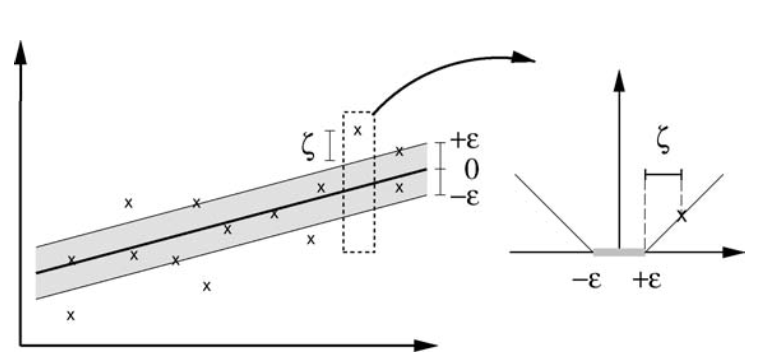
\includegraphics[width=\textwidth]{images/svm_simple.png}    
    \caption{Support vector regression,\cite{learning_with_kernels}}
    \label{fig:svm_simple}
\end{figure}
Smola et al. \cite{smola2004tutorial} point out that considering the dual formulation makes our optimisation problem easier to solve. Doing so we have the equivalent optimisation problem
\begin{equation}
    \begin{aligned}
        \max_{\alpha_i, \alpha_i^*} \quad& -\frac{1}{2}\sum\limits_{i,j=1}^n(\alpha_i-\alpha_i^*)(\alpha_j-\alpha_j^*)\langle x_i,x_j\rangle +\sum\limits_{i=1}^n(\alpha_i-\alpha_i^*)(y_i-\epsilon)
        \\
        s.t. \quad& \sum\limits_{i=1}^n(\alpha_i-\alpha_i^*)=0
        \\
        \quad& \alpha_i, \alpha_i^* \in [0, C]
    \end{aligned}
\end{equation}
Rearranging the gradient of the lagrangian with respect to $w$, we obtain the so called support vector expansion.
\begin{equation}\label{eq:support vector expansion}
    w=\sum\limits_{i=1}^n(\alpha_i-\alpha_i^*)x_i
\end{equation}
This means that $w$ can be completely described as a linear combination of the training features $x_i$.
Notice, the complexity of the function representation is independent of the feature space dimensionality, but depends only on the number of support vectors; that is those point $i$ for which $(\alpha_i-\alpha_i^*)\neq 0$
Moreover, we do not needd to compute $w$ explicitly in order to evaluate $f(x)$.
Furthermore, equation \ref{eq:support vector expansion} implies
\begin{equation}
    f(x)=\sum\limits_{i=1}^n(\alpha_i-\alpha_i^*)\langle x_i, x\rangle +b
\end{equation}
Employing the Karush-Kuhn-Tucker conditions, $b$ can be retrieved easily. Particulalry, the condition that the product between the constraints and the dual variable has to vanish. These implies that the lagrange multipliers $\alpha_i, \alpha_i^*$ may be nonzero only for the samples inside the epsilon insensitive tube. Consequently for any of these data points, the equality $b=y_i-\langle w, x_i-\epsilon\rangle$ holds.
\\
To get an idea of how SVR works, see figure \ref{fig:svr1} for how a support vector regression handles a sinusoidal function with noise.
\\
\begin{figure}
    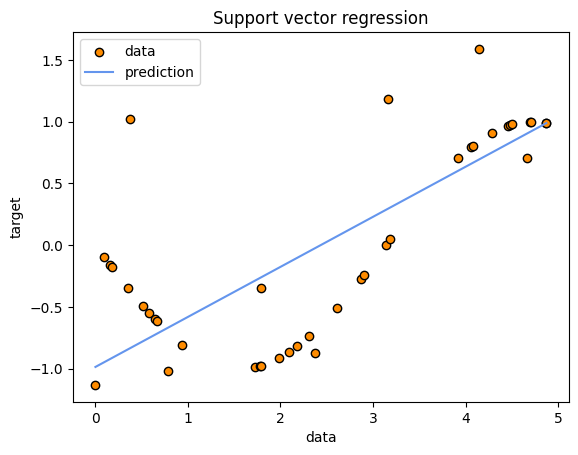
\includegraphics[width=\textwidth]{images/svr1.png}
    \caption{support vector regression}
    \label{fig:svr1}
\end{figure}

\section{Artificial neural networks}
Artificial neural networks (ANN) have been successfully applied in the context of electricity markets forecasting. The basic building block of this class of methods is the perceptron \cite{rosenblatt1958perceptron}.
\begin{equation}
    y=\psi(wx+b)
\end{equation}
where $\psi$ is an activation function and $w,b$ are the parameters of the neuron; such parameters are typically optimized through gradient descent.

\subsection{Multilayer perceptrons}
In order to cover a richer space of models we can stack neurons, doing so we obtain the so called multi layer perceptrons (MLPs). Hyperparameters of these models are the number of hidden layers, the number of neurons in each of those layers and the kind of activation function.
Notice, depending on the numbers of layers, MLPs are sometimes referred to as deep neural networks.

% \subsubsection{NARX}
% Neural networks that have as inputs past values of the target variable and other independent variables are called nonlinear autoregressive exogenous models.

\subsection{Long short term memory}
% https://colah.github.io/posts/2015-08-Understanding-LSTMs/

% https://rtavenar.github.io/deep_book/book_en.pdf
Long short term memory network (LSTM) extends MLP by introducing a cell state in its layers. In this way, the current state of a cell depends on the current value $X_t$, on the previous cell activation and on the previous cell state $C_{t-1}$, see figure \ref{fig:lstm_cell} for a visual representation. 
\begin{figure}[!h]
    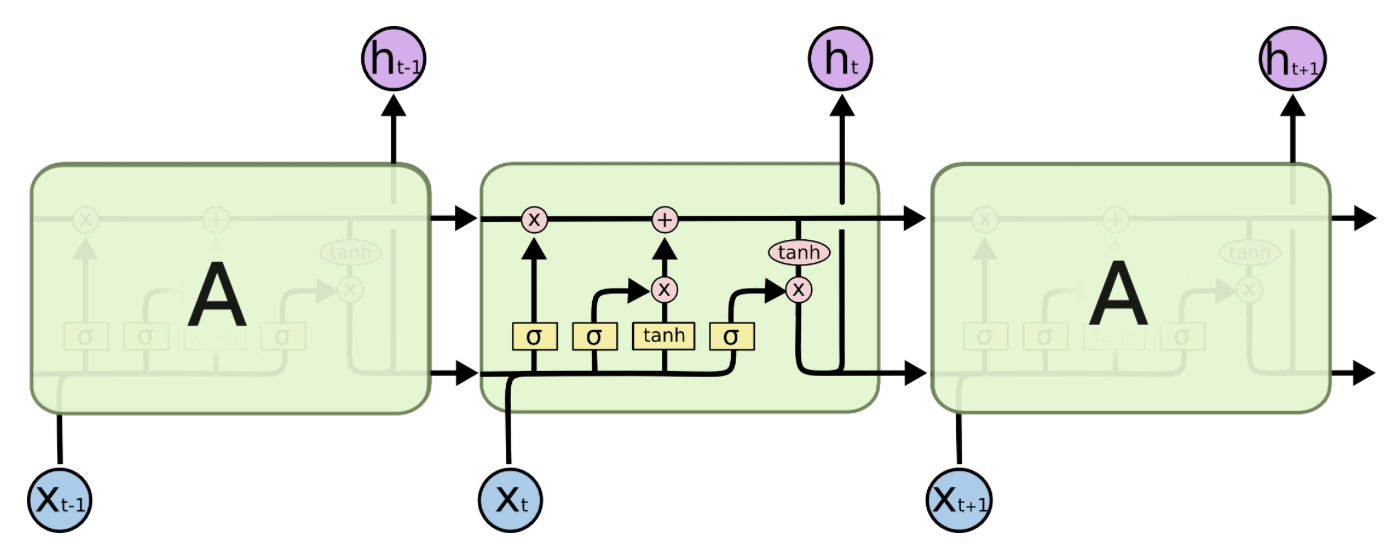
\includegraphics[width=\textwidth]{images/lstm_cell.png}
    \caption{Long short term memory cell}
    \label{fig:lstm_cell}
\end{figure}
The cell is responsible for deciding whether to store/forget long and short term information. To do so, each cell is made of a forget gate, an input gate and an output gate.
The forget gate takes in $h_{t-1}$ and $x_t$ and outputs a real valued vector with elements in the domain $[0,1]$, this corresponds to the ratio of information retention for each element of the cell state $C_{t-1}$.
\\
Its equation is given by
\begin{equation}
    f_t=\sigma(W_f\dot[h_{t-1},x_t]+b_f)
\end{equation}
The input gate is made up of two parts. First, a sigmoid layer decides which values of the cell state will be updated. Second, a tahn layer creates a vector of candidates $\tilde{C}_t$ to add to the current state.
\begin{equation}
    \begin{aligned}
        i_t=&\sigma(W_i\dot[h_{t-1},x_t]+b_i)
        \\
        \tilde{C}_t=&tahn(W_c\dot[h_{t-1},x_t]+b_C)
    \end{aligned}
\end{equation}
The cell state is then updated by
\begin{equation}
    C_t=f_t\odot C_{t-1}+i_t\odot \tilde{C}_t
    % odot is elementwise product
\end{equation}
Finally, we output the current cell state and the tanh activated cell state filtered by the sigmoid layer on the current input and the previous hidden state.
\begin{equation}
    \begin{aligned}
    o_t=& \sigma(W_o[h_{t-1},x_t]+b_o)
    \\
    h_t=& o_t \odot tahn(C_t)
\end{aligned}
\end{equation}
% \subsection{DeepAr} deepar é probabilistic

% \subsection{AR Net} no é un framework non é un metodo

\section{Kernel methods}
\subsection{Kernel ridge regression}
In the setting of kernel ridge regression, we aim at estimating $f$ such that $y=f(x)+\epsilon$. Given a RKHS $\mathcal{H}$, we can estimate $\hat{f}$ by solving the optmisation problem
\begin{equation}\label{eq:kernel ridge}
    \hat{f}=\argmin{f\in \mathcal{H}}\frac{1}{2}\sum\limits_{i=1}^n(y_i-f(x_i))^2+\frac{\lambda}{2}\|f\|_{\mathcal{H}}^2
\end{equation}
Before proceeding, we need to introduce the representer theorem.
\begin{theorem}
    Let $k:\mathcal{X} \times \mathcal{X} \mapsto R$ on a non empty set $\mathcal{X}$ with corresponding RKHS $\mathcal{H}$,
    a strictly increasing real valued function $g:[0,\infty) \to \mathbb{R}$, and $E:(\mathcal{X}\times \mathbb{R}^2)^n \to \mathbb{R} \cup \{\infty\}$.
    Consider the regularized risk functional $Risk[f]:f \mapsto  E\left((x_{1},y_{1},f(x_{1})),\ldots, (x_{n},y_{n},f(x_{n}))\right)+g\left(\| f\| \right)$. Then any minimizer of the empirical risk $Risk[f]$ can be represented as $ f^{*}(\cdot )=\sum\limits_{i=1}^{n}\alpha _{i}k(\cdot ,x_{i})$
\end{theorem}

\begin{proof}
    By orthogonal projection, any $f \in \mathcal{H}$ can be decomposed as the sum of two functions, with the first lying in the $\textrm{span}\{\phi(x_1),\dots, \phi(x_n)\}$ and the second staying in the orthogonal complement of the former. Letting $\nu$ denote a function from the orthogonal complement, we have
    \begin{equation}
        f=\sum\limits_{i=1}^{n}\alpha_i \phi(x_i)+\nu
    \end{equation}
    Applying $f$ to any point, by the reproducing property we have
    \begin{equation}
        \begin{aligned}
            f(x_j)=&\langle \phi(x_j), \sum\limits_{i=1}^{n}\alpha_i \phi(x_i)+\nu\rangle
            \\
            =&\sum\limits_{i=1}^{n}\alpha_i\langle \phi(x_j), \phi(x_i)\rangle
        \end{aligned}
    \end{equation}
    This means that setting $\nu=0$ does not affect the evaluation of $f$.
    Next consider the regularization term; notice, the functional $g$ is defined to be strictly monotonic in order to penalize more complex functions $f$.
    \begin{equation}
        \begin{aligned}
            g(\|f\|)=&g\left(\left\|\sum\limits_{i=1}^n \alpha_i \phi(x_i)+v\right\|_\mathcal{H}\right)
            \\
            =&g\left(\sqrt{\left\|\sum\limits_{i=1}^n \alpha_i \phi(x_i)+v\right\|_\mathcal{H}^2}\right)
            \\
            =&g\left(\sqrt{\left\|\sum\limits_{i=1}^n \alpha_i \phi(x_i)\right\|_{\mathcal{H}}^2+\left\|v\right\|_\mathcal{H}^2+2\langle\sum\limits_{i=1}^n \alpha_i \phi(x_i),\nu \rangle_{\mathcal{H}}}\right)
            \\
            =&g\left(\sqrt{\left\|\sum\limits_{i=1}^n \alpha_i \phi(x_i)\right\|_{\mathcal{H}}^2+\|v\|_\mathcal{H}^2}\right)
            \\
            \geq &g\left(\sqrt{\left\|\sum\limits_{i=1}^n \alpha_i \phi(x_i)\right\|_{\mathcal{H}}^2}\right)
        \end{aligned}
    \end{equation}
    Hence, we can conclude that setting $\nu=0$ decreases the second term while the first term is not affected. Thus it follows that any minimizer of the risk functional of equation \ref{eq:kernel ridge} must be of the following form
    \begin{equation}
        f^*(\cdot)=\sum\limits_{i=1}^n \alpha_i \phi(x_i)=\sum\limits_{i=1}^n \alpha_i k(\cdot, x_i)
    \end{equation}
\end{proof}

Employing the representer theorem, we can rewrite \ref{eq:kernel ridge} in matrix notation as
\begin{equation}
    \begin{aligned}
    \hat{\alpha}=&\argmin{\alpha \in \mathbb{R}^n}\frac{1}{2}\|y-K\alpha\|_2^2+\frac{\lambda}{2}\left\|\sum _{i=1}^{n}\alpha _{i}k(\cdot ,x_{i})\right\|_{\mathcal{H}}^2
    \\
    =&\argmin{\alpha \in \mathbb{R}^n}\frac{1}{2}\|y-K\alpha\|_2^2+\frac{\lambda}{2} \left\langle \sum _{i=1}^{n}\alpha _{i}k(\cdot ,x_{i}),\sum _{j=1}^{n}\alpha _{j}k(\cdot ,x_{j})\right\rangle_{\mathcal{H}}^2
    \\
    =&\argmin{\alpha \in \mathbb{R}^n}\frac{1}{2}\|y-K\alpha\|_2^2+\frac{\lambda}{2} \sum _{i,j=1}^{n}\alpha _{i}\alpha _{j}\langle k(\cdot ,x_{i}),k(\cdot ,x_{j})\rangle_{\mathcal{H}}^2
    \\
    =&\argmin{\alpha \in \mathbb{R}^n}\frac{1}{2}\|y-K\alpha\|_2^2+\frac{\lambda}{2} \sum _{i,j=1}^{n}\alpha _{i}\alpha _{j}K_{ij}
    \\
    =&\argmin{\alpha \in \mathbb{R}^n}\frac{1}{2}\|y-K\alpha\|_2^2+\frac{\lambda}{2} \alpha^\intercal K \alpha
    \\
    =&\argmin{\alpha \in \mathbb{R}^n}\frac{1}{2}(y-K\alpha)^\intercal (y-K\alpha)+\frac{\lambda}{2} \alpha^\intercal K \alpha
\end{aligned}
\end{equation}

Setting the gradient to zero
\begin{equation}
    -Ky+K^2\alpha+\lambda K \alpha\overset{!}{=}0
\end{equation}

We have then, that $\hat{\alpha}=(K+\lambda I)^{-1}y$. It follows that the solution takes the form
\begin{equation}
    \hat{f}(\cdot)=\hat{\alpha}K(\cdot,:)
\end{equation}

\subsection{Kernel support vector regression}
Support vector regression (SVR) can be kernelized by swapping the $\mathbb{R}^n$ euclidean dot product of data $x$ with the dot product in the higher feature space $\mathcal{F}$. Doing so, the optimisation problem can be restated as
\begin{equation}
    \begin{aligned}
        \max_{\alpha_i, \alpha_i^*} \quad& -\frac{1}{2}\sum\limits_{i,j=1}^n(\alpha_i-\alpha_i^*)(\alpha_i-\alpha_i^*)k(x_i, x_j)+\sum\limits_{i=1}^n(y_i-\epsilon)(\alpha_i-\alpha_i^*)
        \\
        s.t. \quad& \sum\limits_{i=1}^n(\alpha_i-\alpha_i^*)=0
        \\
        \quad& \alpha_i, \alpha_i^* \in [0,C]
    \end{aligned}
\end{equation}
Our regressor $f$ is then given by
\begin{equation}
    \begin{aligned}
        f(x)=\sum\limits_{i=1}^n(\alpha_i-\alpha_i^*)k(x_i, x)+b
    \end{aligned}
\end{equation}
Notice, in this setting $w$ is no longer given explicitly. Additionally, with kernel support vector regression we seek for the flattest function in the feature space not the input space.
See figure \ref{fig:svr2} and figure \ref{fig:svr3} for two examples. In the former, we have used a polynomial kernel while in the latter the standard radial basis function kernel.
\begin{figure}
    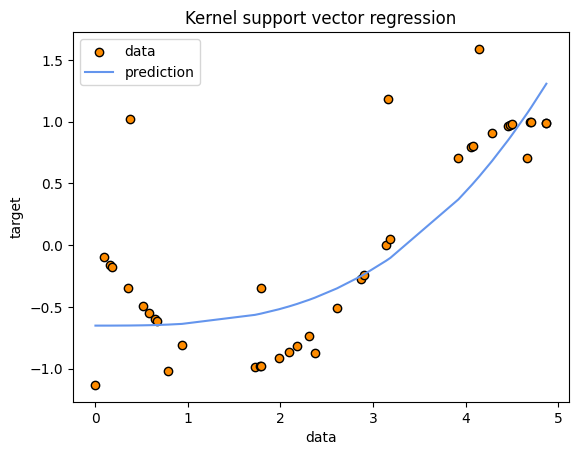
\includegraphics[width=\textwidth]{images/svr2.png}
    \caption{Polynomial support vector regression}
    \label{fig:svr2}
\end{figure}

\begin{figure}
    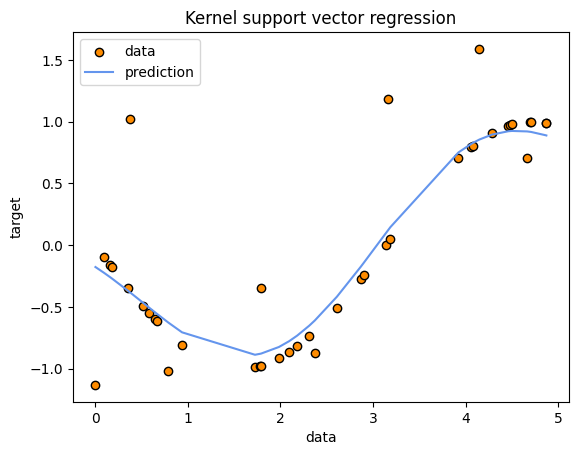
\includegraphics[width=\textwidth]{images/svr3.png}
    \caption{Gaussian RBF support vector regression}
    \label{fig:svr3}
\end{figure}
Comparing theese pictures with figure \ref{fig:svr1}, it can be concluded that introducing kernels allows support vector regression to handle the non linearities in the data.
